\documentclass[11pt]{article}
\usepackage[a4paper, portrait, margin=1in]{geometry}
\usepackage{graphicx}
\usepackage{hyperref}
\usepackage{caption}
\usepackage[labelformat=simple]{subcaption}    %%Adding option to remove parenthesis
\renewcommand{\thesubfigure}{\normalsize Figure \thefigure. (\alph{subfigure}):}
% \usepackage{subcaption}
% \usepackage{subcaption}
%\usepackage{dirtytalk}
\usepackage{float}
\usepackage{eldar_report}
% Useful packages
\usepackage{amsmath}
% \newcommand\norm[1]{\lVert#1\rVert}
\newcommand\normx[1]{\Vert#1\Vert}
\usepackage{graphicx}
\usepackage{lifetime}
\newcommand{\Dana}[1]{\textcolor{purple}{\bf Dana: #1}}
\newcommand{\Julian}[1]{\textcolor{purple}{\bf Julian: #1}}


\begin{document}

\title{Maximal Robust Layer-Neighborhoods in Multi-Label Neural Networks}

\author{
    \textbf{Julian Mour} \\
    \\
    Advisor: Dana Drachsler Cohen\\
    Technion - Israel Institute of Technology
}

\maketitle

%! Author = julianmour
%! Date = 01/05/2023

\section{Introduction}

Multi-label image classifiers are successful in various tasks
\Dana{give at least three examples and include citations.} A multi-label image classifier\Dana{define in one sentence}.
However, many works have demonstrated that deep neural networks (DNNs) are susceptible to adversarial example attacks, e.g.,~\cite{ref7,ref15,szegedy2014intriguing,ref17,ref29,ref56}. These attacks add a small perturbation to a correctly classified input with the goal of causing the network to misclassify.
In particular, several works have shown the vulnerability of multi-label image classifiers \Dana{add at least three citations}.
To understand the robustness level of image classifiers, many verifiers have been introduced \Dana{add many citations}.
However, no verifier analyzes the robustness level of multi-label classifiers. %, where a single instance (e.g.\ an image) is associated with a single label, not mentioning the case of multi-label classifiers where an image can be associated with more than one label.
%The association of two or more labels to a single image can be interesting when it comes to the network's vulnerability to perturbations;
%How can a perturbed object in an image affect the classification of another?

\paragraph{Challenges} Part of the challenge is defining what robustness means in multi-label classifiers.
For (single label) classifiers, a popular definition is \emph{local robustness}. At high-level, given an image classifier, an input to the classifier, and a perturbation limit, the classifier is locally robust if perturbing the given input up to the given limit does not change the network's classification. \Dana{explain why the straight forward extension of the definition is problematic}.
Even given a suitable definition, verifying multi-label classifiers is challenging because they tend to be deeper than single label classifiers\Dana{true?}. \Dana{are there other challenges?}

\paragraph{Multi-label classifier robustness}
In this thesis, we propose a new definition for local robustness of multi-label classifiers. At high level, given a multi-label classifier, an input containing several objects and a perturbation limit, the network is robust if \Dana{complete as in the previous sentence}. This definition allows one to understand: \Dana{complete the motivation to this definition}.
 %want to explore the robustness of different multi-label classifiers in one class - the target class, while adding perturbation around another - the non-target class.

\paragraph{Problem definition} Given \Dana{complete} our goal is to compute\Dana{complete}. A naive optimal algorithm \Dana{complete}. However, it is highly time consuming.

\paragraph{Key idea} To scale the analysis, our key idea is to rely on oracle-guided synthesis\Dana{add citation}. Namely, we propose an algorithm that iteratively expands the specification, given by the series of epsilons\Dana{make sure it's defined in the problem definition paragraph}. At each iteration, a specification is submitted to an existing verifier, capable of analyzing\Dana{complete}. Then, based on its response, we update the specification by numerical optimization, acting as the specification synthesizer.
The synthesizer's challenges are: (1)~the specifications do not adhere to partial order and (2)~computing the gradient is challenging because\Dana{complete}. To cope, we propose to \Dana{complete}.

\paragraph{Preliminary results}
In our preliminary research, we implemented a basic version of the above approach. We evaluate it on the DOUBLE-MNIST test dataset\Dana{add citation}.
We ran our program on three different CNN multi-label DOUBLE-MNIST classifiers that were trained differently: without a defense, with an $L_0$-based defense\Dana{add citation} and with the PGD defense\Dana{add citation}.
Results show that \Dana{complete}.
%We present the results of the program on each classifier and a single image as a heatmap representing the sequence of epsilons - one epsilon per layer.
\paragraph{Future goals}
As part of the thesis, we intend to improve our algorithm by reducing the number of queries to the verifier, and thereby shortening the execution time. To this end, we plan to \Dana{complete how you'll do it}.
We also plan to compute wider robust layer-neighborhoods by \Dana{compelte how you think you'll do it}.
%We also hope to achieve a better understanding of the vulnerability of multi-label classifiers to perturbations and the relation between several class objects in a multi-labeled image.

\Dana{below is the old text need to be rewritten as part of previous paragraphs}

We first build layers around the non-target object in the image.
Each layer can be perturbed by an epsilon (defined specifically for this layer), while maintaining robustness for the target class - not affecting the classification of the target class.
Meaning, we want a sequence of epsilons that for a specific classifier and image, defines a robust layer-neighborhood for the target class.
To get best results, we want the layer-neighborhood to be maximal.
\Dana{this mixes definition and algorithm -- need to separate}

Our key idea is to compute the sequence of epsilons by verifying and optimizing it in each step, rather than computing each epsilon individually.
Given a sequence of epsilons representing an epsilon of perturbation per layer, we check if the layer-neighborhood of a specific image is robust for the target object by running a robustness verifier on it and a specific classifier.
To optimize a robust layer-neighborhood, we compute some gradients in which we can expand our neighborhood and try to keep it robust.
Similarly, we might need to shrink a non-robust layer-neighborhood so that it becomes robust.
The shrinking process can be done in several ways, such as defining a shrinking weight for each layer.
Weights can be fixed (defined by the index of the layer) or not (e.g.\ sensitivity weights).

%! Author = julianmour
%! Date = 01/05/2023

\section{Problem Definition}
In this section, we define the problem we address.
For simplicity's sake, all our definitions and algorithms focus on images with two objects -- the target one and the perturbed one -- but they can extend to multiple objects.
%In general, we can discuss the problem with several target and non-target objects, but for simplicity we will focus on one object from each type.
Informally, given a multi-label classifier, an image showing a target object, we aim to compute a robust layer-neighborhood, given for a target object (target class).
The neighborhood is defined by a sequence of epsilons representing the perturbation per layer.
%Each layer is defined to be a set of pixels that share the same distance from a specific non-target object (non-target class) in the image.
We begin with definitions and then define our problem.
A multi-label classifier is a function mapping an instance, in our case an image from an input domain $\mathbb{R}^{n \times m}$, to a score vector over the possible set of classes $C$,
%\Dana{complete}
$F: \mathbb{R}^{n \times m} \rightarrow {\mathbb{R}}^{|C|}$.
%\\\Dana{is this how you define it in your code? typically there's a score function, and i thought it's also in your case and that there are thresholds. Read Marvel and see how it's defined there}.
%\Dana{complete}.
Given an image $x$, the classification $C'$ of a multi-abel classifier $F$ for $x$ is the subset of $k$ classes with the highest scores,
$C' = \{\arg i^{th}\max_{c' \in C}{F(x)_{c'}\}_{i=1}^{k}$.
In our case and for simplicity's sake $k=2$.
%\Dana{check the previous comment, it should also change, also the classification can't be in term of the target and non target class because it can b any two classes; check how it's defined in Marvel}
%\Dana{complete}.
A neighborhood of input $x$ is a set of inputs $N(x) \subseteq \mathbb{R}^{n \times m}$ containing $x$.
A neighborhood $N(x)$ is robust if all inputs in it are classified to a \textbf{target label} $c_t \in C$, $\forall x' \in N(x): c_t \in \{\arg i^{th}\max_{c' \in C}{F(x)_{c'}}\}_{i=1}^{k}$.\\
%\Dana{fix it accordingly}
%\Dana{complette with words and with mathematical notation}.
We focus on layered neighborhoods.
To define it, we denote the set of pixels showing an object $o$ in an image $x$ by $P_o^x$.
Given an image $x$ showing two objects $o_t$ and $o_{nt}$, the target one with class $c_t$ and the perturbed one with class $c_{nt}$ and its set of pixels ${P_{o_{nt}}^x}$, the $d^\text{th}$ layer is the set of pixels that their Chebyshev distance ($L_\infty$) from ${P_{o_{nt}}^x}$ is $d$.
%\Dana{with respect to what norm?}.
Given two pixels $p = (i,j), p' = (i', j') \in [n]\times [m]$, their distance is $dist(p, p') = ||p - p'||_\infty = \max\{|i - i'|, |j - j'|\}$.
%\Dana{complete. Is it L inf norm?}.
Given a pixel $p = (i, j)\in [n]\times [m]$ and a set of pixels $P \subseteq [n]\times [m]$, their distance is the minimum distance of $p$ to any pixel in $P$: $dist(p, P) = \min\{dist(p, p') \mid p' \in P\}$.
Given an image $x$, an object $o$, and a distance $d$, we define the $d^{th}$ layer:
$l_d^{x,o} = \{p \in [n]\times [m] \mid dist(p, P_o^x) = d\}$.
%Formally, we define the set of layers $L_x$:
%\begin{gather*}
%    L_x = \{l_0^x, l_1^x, \ldots, l_r^x\}\\
%    \textrm{s.t.}  l_d^x = \{(i,j) \in [1,n]\times [1,m] \mid dist((i, j),$ non-target object$) = d\}
%\end{gather*}
Given an image $x$ and a non-target object $o_{nt}$, we define the set of layers by $L_x^{o_{nt}} = \{l_0^{x, o_{nt}}, l_1^{x, o_{nt}}, \ldots, l_r^{x, o_{nt}}\}$, where $r+1$ is the number of layers around $o_{nt}$ covering all pixels in $x$.
%\Dana{what is $r$?it's not defined. is it wrt the target object? the image dimensions?}\Dana{add $P_{NT}$ to layers as superscript}

\paragraph{A layered neighborhood} Given an image $x$, the non-target object's pixels ${P_{o_{nt}}^x}$ and a series of maximal allowed perturbation for every layer $\epsilon=(\epsilon_0,\ldots,\epsilon_r)$, a layered neighborhood ${N^{o_{nt}}_\epsilon}(x)$ is the set of all images whose perturbation at layer $d$ is bounded by the respective perturbation limit:
%\Dana{complete in words and mathematically}.
\begin{gather*}
    {N^{o_{nt}}_\epsilon}(x) = \{x' \in \mathbb{R}^{n \times m} \mid \forall 0\leq d\leq r+1\ \forall (i,j)\in l_d^{x,o_{nt}}: |x'_{i,j} - x_{i,j}|<\epsilon_d\}
\end{gather*}

We also denote the set of all robust layered neighborhoods of an image $x$ with $RLN_x$, and the set of epsilon sequences representing them with $RES_x$.\\

%\Dana{it's not how we need to define it, see how we define the problem in Marvel}
Given a weight vector $w = (w_0, w_1, \ldots, w_r)$ assigning a weight for each layer, the size of a layered neighborhood ${N^{o_{nt}}_\epsilon}(x)$ is $||{N^{o_{nt}}_\epsilon}(x)|| = w \times \epsilon^T = \sum_{d=0}^{r}{w_d \cdot \epsilon_d}$.\\
%\Dana{complete}.

Now we can define our problem:
Given a classifier $F: \mathbb{R}^{n \times m} \rightarrow {\mathbb{R}}^{|C|}$, an image $x \in [0,1]^{n \times m}$ containing two objects: $o_t$ and $o_{nt}$ \textrm{s.t.} $C' = \{\arg i^{th}\max_{c' \in C}{F(x)_{c'}\}_{i=1}^{k} = \{c_t, c_{nt}\}$,
the goal is to compute a sequence of epsilons $\epsilon^* = ({\epsilon_0}^*, {\epsilon_1}^*, \ldots, {\epsilon_r}^*)$ satisfying:

\begin{enumerate}
    \item $F$ is robust at ${N^{o_{nt}}_{\epsilon^*}}(x)$.
    \item For every $\epsilon'$ expanding $\epsilon^*$, ${N^{o_{nt}}_{\epsilon'}}(x)$ is not robust.
    \item ${N^{o_{nt}}_{\epsilon^*}}(x)$ maximizes its size among all layered neighborhoods meeting (1) and (2).
\end{enumerate}

%\begin{gather*}
%    \varepsilon_x^*  = argmax_{\varepsilon_x \in RLN_x^\varepsilon} \{w_x \times \varepsilon_x^T\}\\
%%    I_x = \{x' \mid \forall l_d^x\in L_x: \forall (i,j)\in l_d^x: x'_{i,j} \in [x_{i,j}-\varepsilon_d^x, x_{i,j}+\varepsilon_d^x]\}\\
%\end{gather*}
%\Dana{fix the above so it will be like in Marvel}
%\Dana{comment 1: don't put \$ in gather env}
%\Dana{comment 2: we don't build programs, but rather algorithms}
%\Dana{comment 3: in this section, we aim to compute maximal neighborhoods, not design an algorithm, this will come in the nxt section}

%! Author = julianmour
%! Date = 01/05/2023

\section{Our Approach}

In this thesis, we will design an algorithm that given a multi-label classifier and an image computes the maximal neighborhood given by an epsilon sequence, describing how perturbation of the non-target object affects the classification of the target object.
A naive algorithm computes the epsilon series one by one, where at each iteration it computes the maximal epsilon using a binary search.
However, this approach is suitable in case the weight vector poses a strict ordering on the importance of the layers, and it also has a high time overhead.
%Problem is this approach is very expensive in time hence inefficient.
Instead, we aim to build on the oracle-guided numerical verification proposed in~\cite{MARVEL}, to obtain a scalable algorithm.
Technically, our algorithm has three main components, that iteratively interact with one another:
\begin{itemize}
    \item A local robustness verifier: Given a classifier and a layered neighborhood ${N^{o}_\epsilon}(x)$ of an image $x$ and object $o$, it determines whether the classifier is robust in this neighborhood.
        \item A numerical optimizer: Given a classifier and a robust layered neighborhood, it attempts to expand the neighborhood into a larger robust neighborhood, with respect to the weight vector. %by expanding it more, as we intend to maximize the norm of the neighborhood.
    \item A counterexample-guided inductive synthesiser (CEGIS): Given a classifier and a \emph{non-robust} layer-neighborhood, it attempts to identify directions of the previously robust neighborhood that cannot be further expanded. 
    \end{itemize}
The components interact until the neighborhood cannot be further expanded.
We next provide details about the different components and explain the open challenges.

    \paragraph{The verifier}
    There are many verifiers that can reason about the local robustness of a (single-label) classifier.
    However, none addresses a multi-label classifier.
    Thus, part of the challenge is adapting a verifier to multi-label classification.
    In particular, the verifier only has to prove that one of the labels is the target object's label. %Since this is a multi-label classifier, we are interested only in the target class robustness;
    %The verifier will say that the neighborhood is robust if and only if all images in the neighborhood are classified to the target class.
    In our preliminary research, we rely on the mixed-integer linear program (MILP) based verifier, called MIPVerify~\cite{MIPVERIFY}.
    This verifier encodes the robustness task into a MILP maximization problem and uses the Gurobi Optimizer to solve it.
    We adapt the verifier to multi-label classifiers by adapting the objective function.
    For a single-label classifier, the objective function is the difference between the highest score and the score of the target class:
    \begin{gather*}
        \max_{c \in C, c \neq c_{t}}\{F(x')_c- F(x')_{c_{t}}\mid x'\in N(x)\}
    \end{gather*}
    If the difference is negative, the neighborhood is robust. Otherwise, it is not robust.
    We call inputs in $N(x)$ maximizing this objective function the \emph{weakest points}, because they are the closest to the decision boundary.
%     A negative value of the maximized objective indicates a robust neighborhood.

    We adapt this objective function to multi-label classifiers as follows.
    Since classification is a set of the classes, instead of comparing to the highest score, we compare to the second highest score:
    %Meaning that the objective now represents the difference between the second-highest score of an incorrect class and the score of the target class ($c_{t}$).
    \begin{gather*}
        2^{nd}\max_{c \in C, c \neq c_{t}}\{F(x')_c- F(x')_{c_{t}}\mid x'\in N(x)\}
    \end{gather*}
    A negative value indicates that the neighborhood is robust with respect to $c_t$.
    %Beyond determining whether a neighborhood is robust or not, the verifier returns a set of points maximizing the objective, to which we call \emph{the weakest points of the image}.
    As before, the inputs maximizing this objective are called the weakest points.
    These points later help the optimizer to identify robust directions to expand the current neighborhood.
    %These are the points in the checked neighborhood that are least robust and the verifier will pass them to the optimizer as well.
    
    \paragraph{The optimizer}
    Our optimizer follows the approach of~\cite{MARVEL} and expands a robust neighborhood by computing the gradient of the optimization problem defined in the previous section.
    Since it is a constrained optimization, we relax the constraints and add equivalent terms to the optimization goal, similarly to ~\cite{MARVEL}.
    %We call this term \emph{the robustness level} (RL).\Dana{to define it, you need to present here the optimization function corresponding to the one on page 7 before}
    %To expand a robust neighborhood, our optimizer 
    %computes the gradients of both terms.
    %The norm's gradient is computed in a straightforward way while the RL's gradient is computed using the weakest points found by the verifier.
    Given the gradients, the optimizer expands the neighborhood by a small step and submits to the verifier. 
%    \Dana{is there an adaptation to mulit-label or is it like Marvel? we need to describe it}
%    \Julian{No adaptation in this part}
    %At last, we calculate the step gradient, which is a combination of both previous gradients, and expand the neighborhood towards the step gradient.
    
    \paragraph{The CEGIS component}
    The CEGIS component takes a non-robust neighborhood and the previously robust neighborhood and attempts to identify directions that must be shrunk towards making the (non-robust) neighborhood robust. %If the neighborhood checked by the verifier isn't robust, then we skip the optimization part.
    %Instead, we try to minimally shrink the neighborhood so that its robust.
    Computing the exact directions requires an exponential number of queries to the verifier.
    Instead, we shrink the non-robust neighborhood in the direction of the previously robust neighborhood.
    In our preliminary research,
    we shrink each layer according to a given weight vector, called \emph{the cutting weight}, which may depend on the input: $cw_x = (cw_0^x, cw_1^x, \ldots, cw_r^x)$.
    %The layer's cutting weight determines how much should the layer be shrunk towards the previously robust neighborhood.
    %We notate the cutting weights vector with $cw_x$, and its complement vector with $cw_x^*$ and define it as follows:
%    \Dana{what is a cutting vector? you need to first provide a high level explanation before the math notation};
    %\begin{gather*}
    %    cw_x = (cw_0^x, cw_1^x, \ldots, cw_r^x)\\
    %    cw_x^* = (1 - cw_0^x, 1 - cw_1^x, \ldots, 1 - cw_r^x)\\
    %\end{gather*}
    Mathematically, this translates to computing a new epsilon sequence $\varepsilon_x'$ that is a weighted average of the current non-robust epsilon sequence $\varepsilon_x$ and the previously robust neighborhood $\varepsilon_x^*$.
    We use \emph{element-wise multiplication} ($\odot$) to multiply each element in the epsilon sequences with its corresponding weight in the weights vectors:
%    \Dana{we cannot place all math notation together; please fix it so it looks like the previous section}.
    $
        {\varepsilon_x}' = \varepsilon_x \odot cw_x^T + \varepsilon_x^* \odot {cw_x^{-1}}^T
    $, where $ cw_x^{-1} = (1 - cw_0^x, 1 - cw_1^x, \ldots, 1 - cw_r^x)$. 
%    \Dana{what is the $\odot$ operation?}
    We consider two definitions for the cutting weights:
    \begin{itemize}
        \item Fixed weights shrinking the neighborhood more in layers that are far from the non-target object and less in layers that are close to it:
        \begin{gather*}
            cw_x = ({\frac{r}{r+1}}^5, {\frac{r-1}{r+1}}^5, {\frac{r-2}{r+1}}^5, \ldots, 0)
        \end{gather*}
%        \Dana{not clear, can you define it mathematically?}
        \item Sensitivity weights shrinking more in layers that are less sensitive to perturbations.
        The sensitivity weights of an image are computed by using the Vanilla Gradient method, introduced by Simonyan et al.~\cite{VANILLAGRADIENT}.
        This method computes the sensitive pixels in an image by computing the gradient of a loss function with respect to the image pixels using backpropagation.
        Pixels with large gradients are likely to be more sensitive to perturbations, and perturbing them is likely to affect the classifier's robustness more.
        We translate the problem of finding sensitive pixels to finding sensitive layers by averaging all pixels' gradients in each layer.
        Accordingly, we define the cutting vector
        $cw_x = (sw_0^x, sw_1^x, \ldots, sw_r^x)$,
        where $sw_i^x < sw_j^x$ implies that layer $i$ is more sensitive to perturbations than layer $j$.
%       \Dana{please describe in high level what it means sensitivity and the vanilla graident approach}
%       \Dana{same comment, this part is important because it's the novel part}
    \end{itemize}
%    Then, the optimizer is given \Dana{complete}. %The new layer-neighborhood will be the input of the verifier in the next iteration.

%Like that, we do this in iterations many times until convergence of the layer-neighborhood and the RL\@.
%We aim to reach a maximal robust layer-neighborhood at the end of the process.


%! Author = julianmour
%! Date = 01/05/2023

\section{Preliminary Results}
We evaluated our preliminary approach on the Double-MNIST dataset, consisting of images showing two digits.
The multi-classifier's goal is to return the correct two digits. % from ten classes;
%$C = \{0, 1, \ldots,9\}$ (the 10 different digits), each image classified to two different classes (contains two different digits).
An example of an image is shown in Figure~\ref{fig:double-mnist-sample}. %, where the digit $4$ is the target object and the digit $9$ is the non-target object.
\begin{figure}
\centering
\begin{minipage}{.4\textwidth}
  \centering
  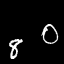
\includegraphics[width=0.6\linewidth]{108_80.png}
  \captionof{figure}{A Double-MNIST sample.}
   \label{fig:double-mnist-sample}
\end{minipage}%
\begin{minipage}{.6\textwidth}
  \centering
  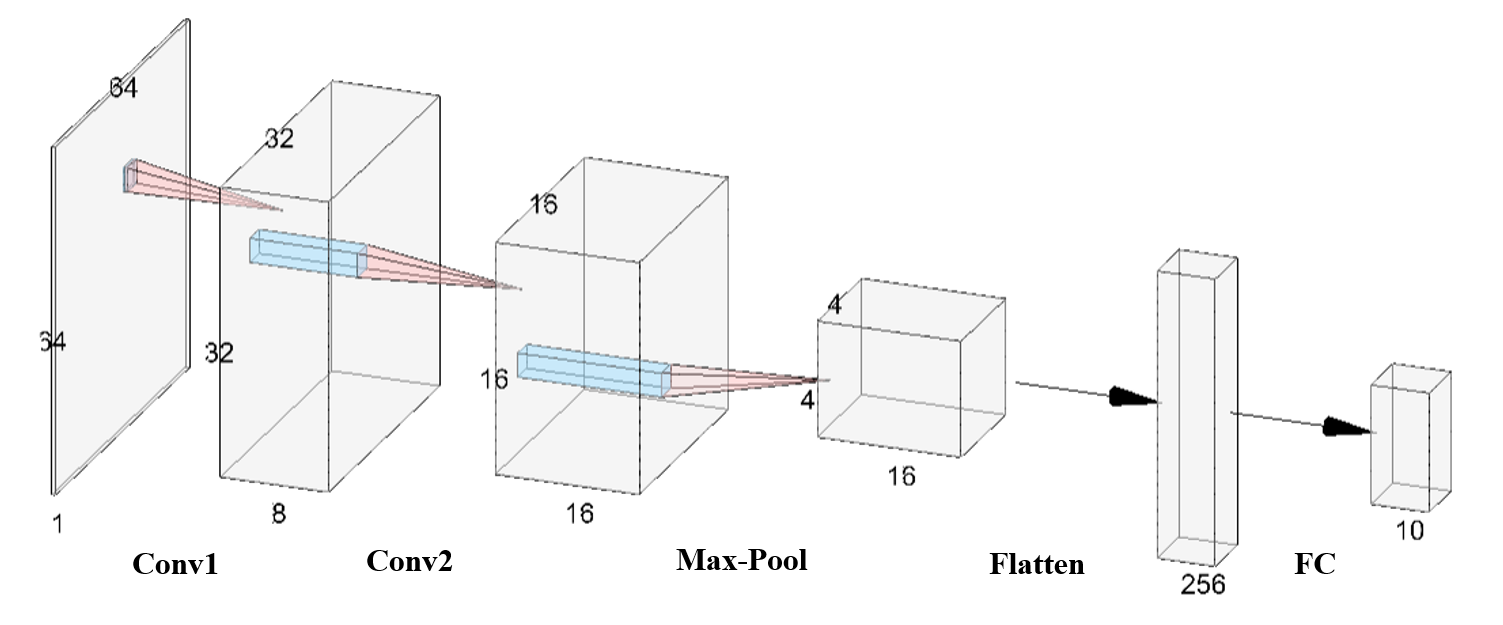
\includegraphics[width=1\linewidth]{arch_labeled.png}
  \captionof{figure}{The classifiers' architecture.}
  \label{fig:arch_labeled}
\end{minipage}
\end{figure}
We ran our algorithm on three different CNN multi-label DOUBLE-MNIST classifiers, all with the same architecture (shown in Figure~\ref{fig:arch_labeled}) but a different training procedure:

%\Dana{describe it and how many neurons}
%While the three of them solve the same classification problem, they differ in their training process:
\begin{itemize}
    \item Without defense. %- This network is trained regularly on the original DOUBLE-MNIST training dataset, without additional processing done to the training dataset.
      \item With an $L_0$ defense: This defense relies on the following data augmentation.
    Before forwarding a training sample to the network, we add random noise to the image in the form of a black rectangle.
        \item With an $L_{\infty}$ defense: Using the Projected Gradient Descent (PGD) defense~\cite{PGD}.
    This defense also involves training the model with adversarial examples, but unlike the $L_0$ defense, the added perturbations are a small value and can be anywhere in the input.
    %The PGD generated adversarial examples are achieved by trying to increase the model's loss function as much as possible.
    %Therefore, training the model with such adversarial examples should make the network more robust.
\end{itemize} 

To compare between the robustness of the models, we ran our algorithm on each of them, for a set of 30 images $X$.
We run our algorithm twice, once for each cutting weights type (fixed and based on sensitivity).
We measure the average unweighted neighborhood size defined as $\sum_{i=0}^{r}{{\epsilon_i}^*}$.
%$\frac{\sum_{x \in X}{||{N^{o_{nt}}_\epsilon}(x)||}}{|X|}$ (see Paragraph~\ref{par:layeredneighborhood}).
%\Dana{complete the math computation}.
We also measure the average execution time for a single image, which is about 75 minutes, but can reach up to 4 hours for big neighborhoods.
%\Dana{complete}.
\begin{figure}
    \centering
    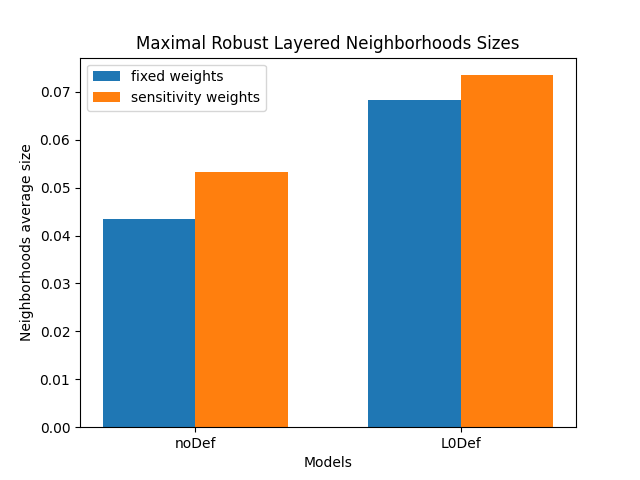
\includegraphics[width=0.7\textwidth]{neighborhoods_average_size.png}
    \caption{The average size of the synthesized neighborhoods.}
%    \Dana{remove the title "Maximal robust..."}
    \label{fig:neighborhoods_average_size}
\end{figure}
Figure~\ref{fig:neighborhoods_average_size} shows the average neighborhood size for each model and each cutting weights type.
The result show that, as expected, the defended models are more robust and the $L_{\infty}$ defended model is the most robust.
This is expected because our attack model focuses on the $L_{\infty}$ norm.
 The results further show that using sensitivity weights as cutting weights enable our algorithm to synthesize larger robust neighborhoods.
%The average size of the neighborhoods returned by our program is presented in Figure~\ref{fig:neighborhoods_average_size}.
%

%\Dana{complete}.
    \begin{figure}
         \centering
         \begin{subfigure}[b]{0.4\textwidth}
             \centering
             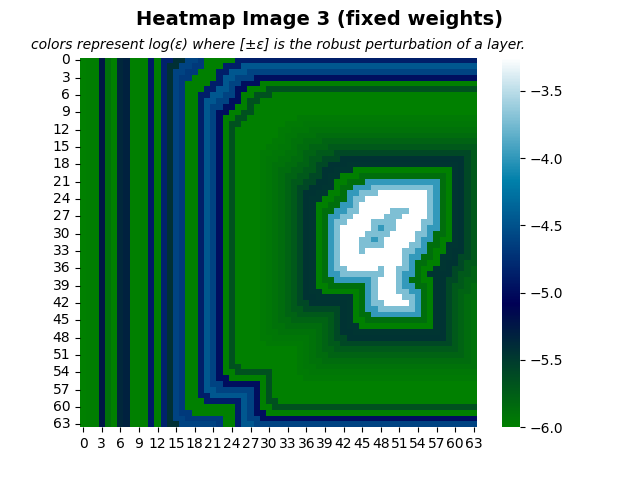
\includegraphics[width=\textwidth]{no_defense_fixed_weights.png}
             \caption{fixed weights}
             \label{sub-fig:No defense FW}
         \end{subfigure}
         \hfill
         \begin{subfigure}[b]{0.4\textwidth}
             \centering
             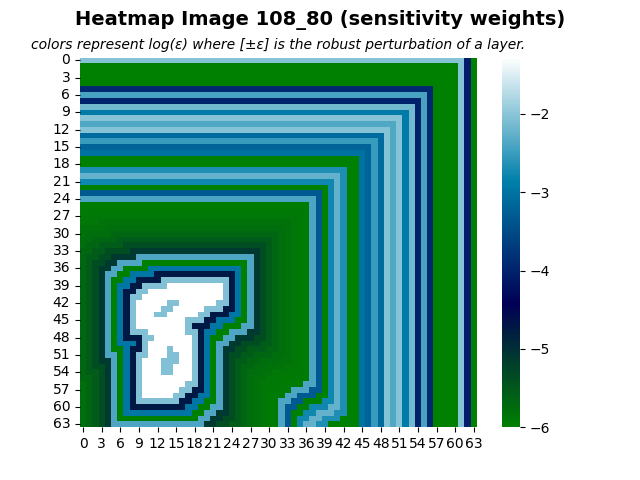
\includegraphics[width=\textwidth]{no_defense_sensitivity_weights.png}
             \caption{sensitivity weights}
             \label{sub-fig:No defense SW}
         \end{subfigure}
         \caption{No Defense}
         \label{fig:No defense}
     \end{figure}
    % In Figure~\ref{fig:L0 defense} we present results of our program ran on a classifier trained with $L_0$ defense, and a single image, as a heatmap representing the epsilons per each layer.
    \begin{figure}
         \centering
         \begin{subfigure}[b]{0.4\textwidth}
             \centering
             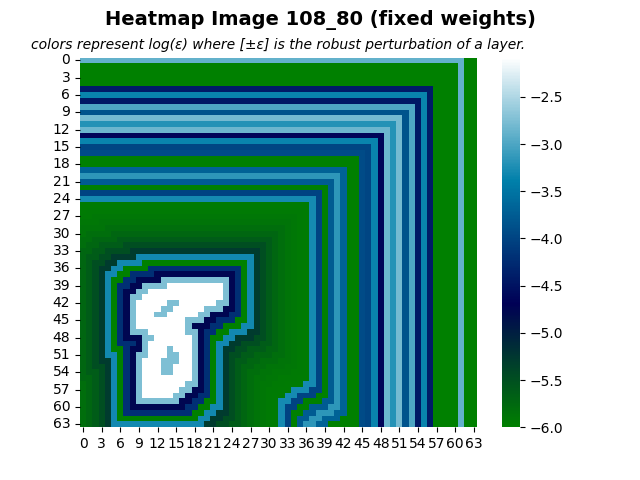
\includegraphics[width=\textwidth]{l0_defense_fixed_weights.png}
             \caption{fixed weights}
             \label{sub-fig:L0 defense FW}
         \end{subfigure}
         \hfill
         \begin{subfigure}[b]{0.4\textwidth}
             \centering
             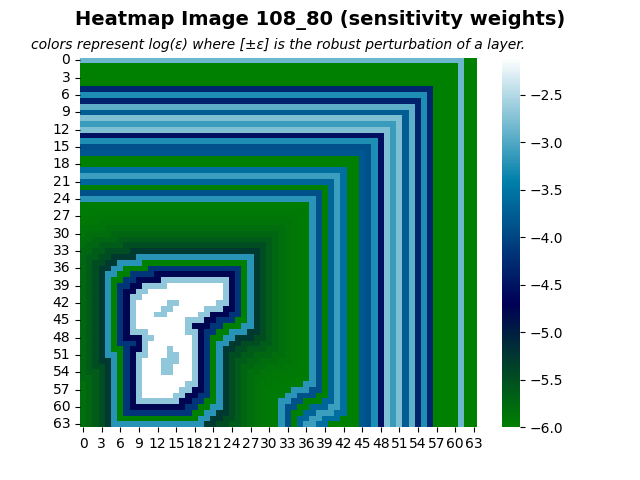
\includegraphics[width=\textwidth]{l0_defense_sensitivity_weights.png}
             \caption{sensitivity weights}
             \label{sub-fig:L0 defense SW}
         \end{subfigure}
         \caption{$L_0$ Defense}
         \label{fig:L0 defense}
    \end{figure}
    \begin{figure}
         \centering
         \begin{subfigure}[b]{0.4\textwidth}
             \centering
             \includegraphics[width=\textwidth]{lInf_defense_fixed_weights.png}
             \caption{fixed weights}
             \label{sub-fig:LInf defense FW}
         \end{subfigure}
         \hfill
         \begin{subfigure}[b]{0.4\textwidth}
             \centering
             \includegraphics[width=\textwidth]{lInf_defense_sensitivity_weights.png}
             \caption{sensitivity weights}
             \label{sub-fig:LInf defense SW}
         \end{subfigure}
         \caption{$L_{\infty}$ Defense}
         \label{fig:LInf defense}
    \end{figure}

Figure~\ref{fig:No defense} demonstrates the difference between the types of the cutting weights.
  For a given image, the undefended classifier and a cutting weight type, we show the heat map corresponding to synthesized layered neighborhood.
  Figure~\ref{fig:L0 defense} is similar but for the $L_0$ defended network.
  Figure~\ref{fig:LInf defense} is similar but for the $L_{\infty}$ defended network.
  In all models, the heat maps show a slightly bigger neighborhood when using the sensitivity weights method, matching our expectations.
  We also see bigger epsilons for layers closer to the non-target object, matching the chosen weight vector defining the size.

%! Author = julianmour
%! Date = 01/05/2023


\section{Future Research Objectives}
In light of the preliminary work, we aim to further explore our ideas in the following directions:
\begin{itemize}
    \item Reduce the number of queries to the MILP verifier, and generally reduce the execution time:
    A main challenge in our current algorithm is the computation of the weakest points.
    This idea has been adapted from~\cite{MARVEL}, focusing on single label classifiers.
    In this setting, this computation involves at most $|C|$ queries per iteration to the MILP solver.
    In our setting, it involves  $|C|^2$ queries per iteration.
    This leads to a very high execution time.
    To reduce the number of queries, we plan to use incomplete verifiers (see Section~\ref{subsec:verifiers}) in some queries, 
    which are faster.
    We plan to also reduce the number of queries from $|C|^2$ via mathematical considerations.
%    \Dana{complete}.
    \item Increase the size of the robust neighborhoods: The size of the returned neighborhood depends on the optimizer and the CEGIS component.
    To increase the size, we aim to develop optimal cutting weights that minimally shrink a non-robust neighborhood to make it robust.
    We plan to also investigate ways to identify layers that can expand more at the expense of others, with the goal of increasing the neighborhood size.
%    \Dana{complete}
     %This can be affected by many factors (e.g.\ the shrinking method used in the algorithm) - we will explore each of these factors and look for the best methods to achieve this goal.
\item Consider more complex datasets: In our preliminary research, we focus on the Double-MNIST dataset. In our research, we plan to consider more complex datasets, e.g., ones showing road images. 
    \item Infer explanations: Our algorithm finds a relation between two objects in a given image and a given multi-label classifier.
    We aim to generalize the relations to infer explanations on the robustness level of a multi-label classifier. The explanations can tell us how much and where we can perturb an image without affecting the classification of the target object. 
%    These can vary between different classifiers as well, which will also help us understand which type of multi-label networks are most vulnerable to perturbations in different locations in their inputs.
\end{itemize}


%! Author = julianmour
%! Date = 01/05/2023

\section{Related Work}
Our thesis is related to neural network verification, adversarial attacks against multi-label classifiers, and counterexample-guided synthesis.

\subsection{Neural Network Verification}\label{subsec:verifiers}
Neural network verifiers analyze safety properties of neural networks.
These verifiers rely on different mathematical techniques, such as constraint solving and model checking, to analyze the behavior of neural networks and determine whether the given property holds.
There are various neural network verification techniques, such as abstract interpretation (e.g.~\cite{ABSTRACTINTER, INCOMPLETE1}), mixed-integer linear programming (e.g.~\cite{MIPVERIFY, singh2018robustness, lazarus2022mixed}), over-approximation analysis (e.g.~\cite{qin2019verification, overapprox, NEURIPS2018_2ecd2bd9}) and in particular over-approximation by linear relaxations (e.g.~\cite{NEURIPS2021_fac7fead, Boopathy_Weng_Chen_Liu_Daniel_2019, 8418593, NEURIPS2019_0a9fdbb1, NEURIPS2019_246a3c55, linearOverapprox, MLSYS2021_ca46c1b9}), simplex (e.g.~\cite{Reluplex, Marabou, simplex-based}) and duality (e.g.~\cite{raghunathan2020certified, dvijotham2018dual}).
%\Dana{add more, see Marvel}
Two main categories of verifiers are:
\begin{itemize}
    \item Complete verifiers: return a definite answer whether a given property, such as neighborhood robustness, holds or not~\cite{MIPVERIFY, COMPLETE}.
    Such verifiers tend to have long execution time and thus do not scale to large networks.
        In our preliminary research, we rely on a complete verifier~\cite{MIPVERIFY}.
    \item Incomplete verifiers: may also return \emph{unknown} for a given property.
    This allows them to rely on approximate techniques which scale better~\cite{INCOMPLETE1, INCOMPLETE2}.
\end{itemize}

\subsection{Adversarial Attacks in Multi-Label Classification}
In an adversarial attack, an adversary intentionally perturbs an input to the classifier to cause misclassification.
In multi-label classification, each input can be assigned multiple classes.
Adversarial attacks in this setting can be defined with respect to various goals, such as causing the classifier to predict a different incorrect subset of classes or not predicting a given correct class.
We focus on the latter goal, also known as untargeted attack.
%Most existing works on adversarial attacks have been focused on the case of multi-class single-label classification~\cite{SINGLElABEL1, SINGLElABEL2, SINGLElABEL3, SINGLElABEL4}.\Dana{is the previous sentence related to us? we are in multi label no?}
%Several others on the case of multi-label classification, where attacks are mainly divided to two types: \textbf{(1)~Targeted Attacks} - aim to bring specific incorrect labels' scores to be the highest and \textbf{(2)~Untargeted Attacks} - aim to bring the correct labels' scores to not be the highest.
%Our property focuses on giving a robust neighborhood against a type of untargeted attacks;
%Such attacks that aim to bring a specific correct label's score to not be in the top picked labels.
    Song et al.~\cite{MULTIlABEL1} introduce targeted white-box attacks for multi-label classification.
    They propose a method to exploit label-ranking relationships based framework to attack multi-object ranking algorithms.
    They approach the problem by formulating it as an optimization problem that meets the attack target while ensuring that the perturbation will not be too obvious, and then execute gradient descent.
    Through experimentation, they discover that they could manipulate a multi-label classifier into producing any set of labels for a given input by adding an adversarial perturbation.
%    \Dana{what is the discovery? sounds like a solution to their optimization function}.
    Zhou et al.~\cite{MULTIlABEL2} suggest generating $L_{\infty}$-norm adversarial perturbations to trick multi-label classifiers.
    They solve the problem by transforming the optimization problem of finding adversarial perturbations into a linear programming problem, which can be solved efficiently.
    Yang et al.~\cite{MULTIlABEL3} explore the potential for misclassification risk in multi-label classifiers, particularly in worst-case scenarios.
    They approach the problem by formulating it as a bi-level set function optimization problem and use random greedy search to find an approximate solution.
    More recently, Hu et al.~\cite{Hu_2021_ICCV} present a method to disrupt the top-$k$ labels of multi-label classifiers, based on novel loss functions, under both untargeted and targeted attacks.
    Melacci et al.~\cite{melacci:hal-02971233} suggest a multi-label attack approach with a domain knowledge-constrained classifier, where the domain knowledge is on the relationship of the considered classes.
    This approach enables the prediction of adversarial examples within the distribution of the training data.
    Kong et al.~\cite{9857594} were the first to develop a differential evolution (DE) algorithm that can effectively generate multi-label adversarial examples.
    They achieve a black-box attack that does not need to access model parameters and only uses the model's outputs to generate adversarial examples.
    Mahmood et al.~\cite{mahmood2022effective} take into consideration label relationships, modeled by a knowledge graph.
    They propose a graph-consistent multi-label attack framework, which searches for small image perturbations that lead to misclassifying a desired target set while respecting label hierarchies.
%\Dana{there are only three works? we need at least six and ideally ten if there are.}
%\Julian{Added 4 more works (7 in total). Tried finding more but found them less relevant.}

\subsection{Counterexample-Guided Synthesis}
Counter example guided synthesis (CEGIS) is a technique used in formal verification and program synthesis to generate correct programs or system designs for given specifications.
CEGIS iteratively searches for a candidate, checks with an oracle whether the candidate satisfies the specification, and if not relies on counterexamples to refine the search space and guide the synthesis process.
In this research, we use CEGIS to recover the search for a robust neighborhood after reaching a non-robust neighborhood. %desired epsilons sequence that will define a robust maximal layer-neighborhood;
In our context, the specification is a robust layer-neighborhood, the oracle is the verifier, and the counterexamples are the weakest points.
%We submit several queries to a verifier in each iteration and update the epsilons sequence accordingly, given the counterexamples.
Previous work also used CEGIS to find maximal robust neighborhoods~\cite{CEGIS1, MARVEL, CEGIS2, CEGIS3}. %, we use similar approach as MaRVeL's~\cite{MARVEL}. 


\bibliography{bibliography}
\bibliographystyle{plain}

\end{document}
